\begin{figure}[t]
\centering
% 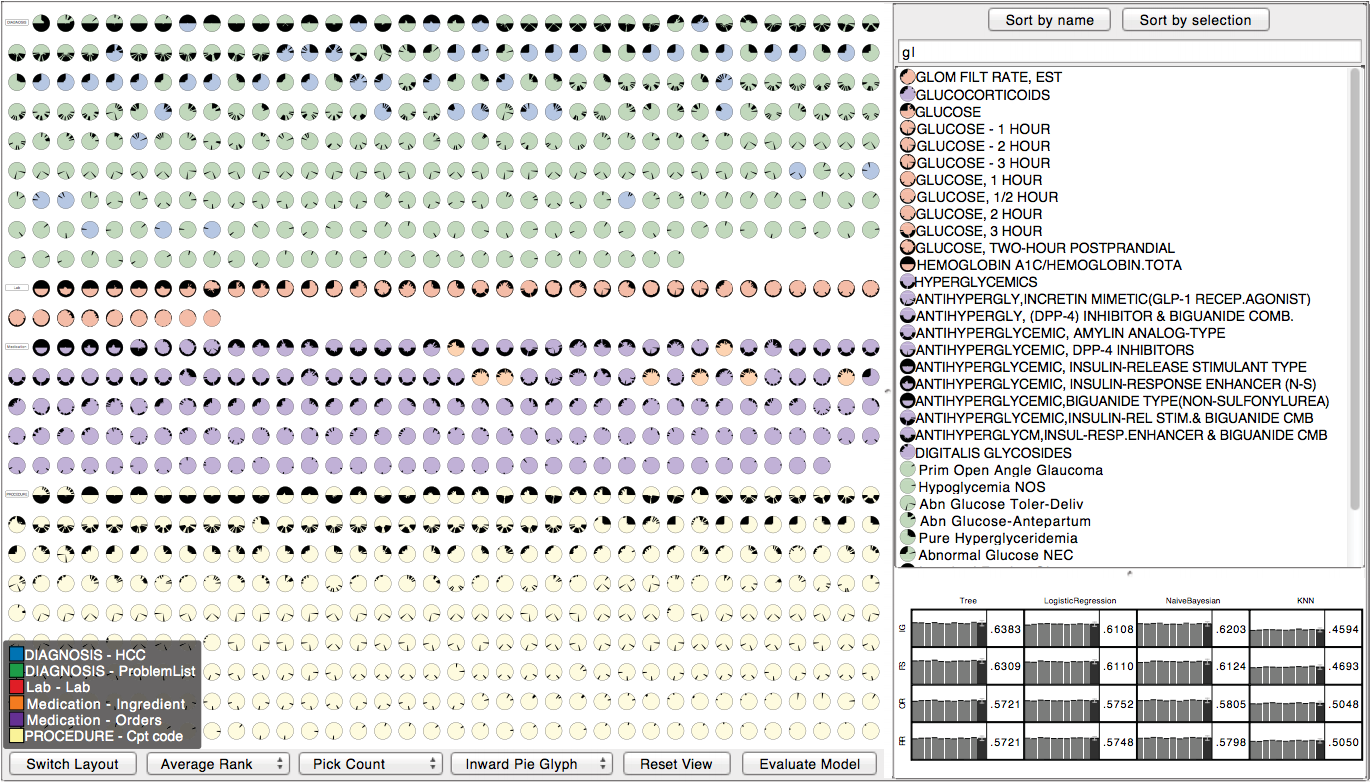
\includegraphics[scale=0.32]{fig/overview}
% ~
% \includegraphics[scale=0.32]{fig/confusion}
% ~
% 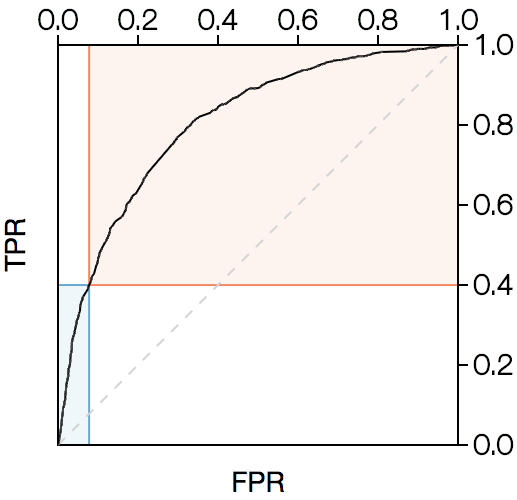
\includegraphics[scale=0.32]{fig/roc}
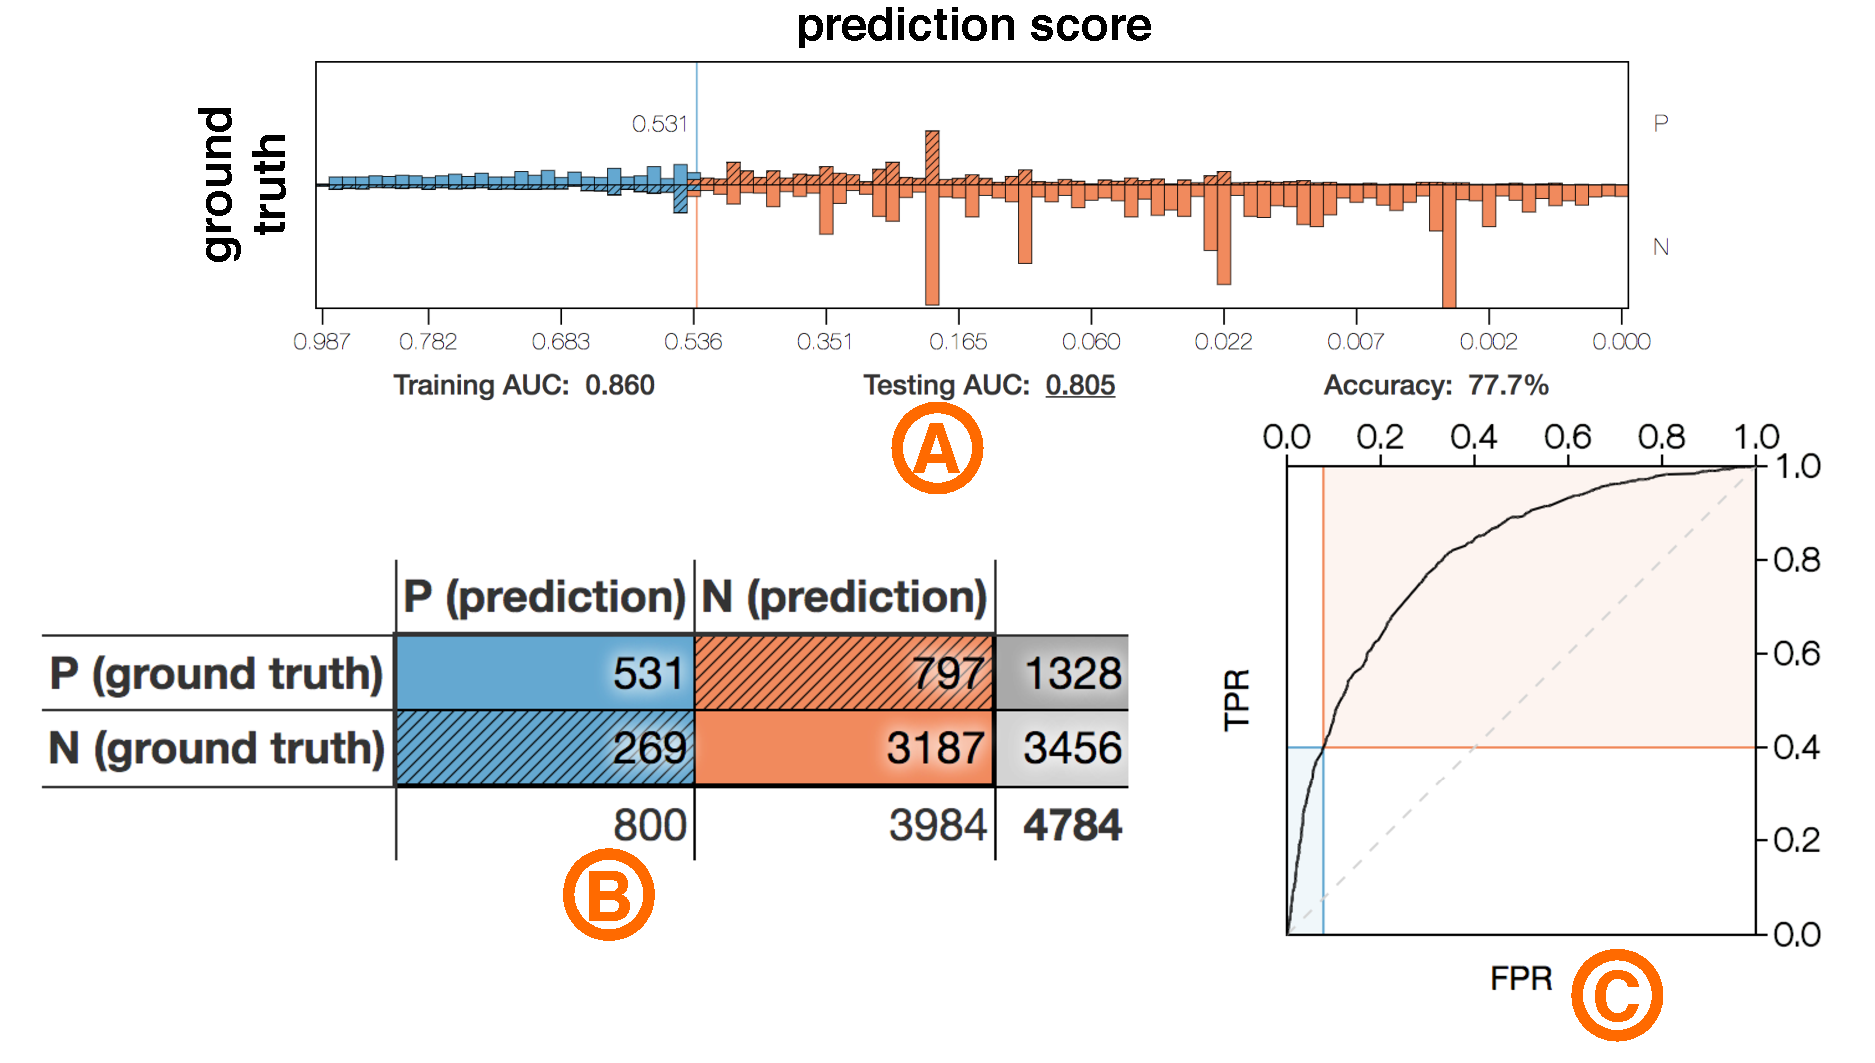
\includegraphics[width=\columnwidth]{explainer/overview_final}
\vspace{-8mm}
\caption{
The \textbf{\tabA}.
(A) Histograms showing the distribution of prediction scores.
The direction of the bars indicates the ground truth and their position relative to the threshold line (at 0.531) indicates the predicted label.
(B) The confusion matrix shows the number of correct and incorrect predictions. (C) The ROC curve shows the prediction quality.
}
\vspace{-5mm}
\label{figs:overview}
\end{figure}

% Selecting the peak left of 0.165 reveals ``Sodium Chloride" as its main cause in the \tabB. 